% Options for packages loaded elsewhere
\PassOptionsToPackage{unicode}{hyperref}
\PassOptionsToPackage{hyphens}{url}
%
\documentclass[
]{article}
\usepackage{amsmath,amssymb}
\usepackage{iftex}
\ifPDFTeX
  \usepackage[T1]{fontenc}
  \usepackage[utf8]{inputenc}
  \usepackage{textcomp} % provide euro and other symbols
\else % if luatex or xetex
  \usepackage{unicode-math} % this also loads fontspec
  \defaultfontfeatures{Scale=MatchLowercase}
  \defaultfontfeatures[\rmfamily]{Ligatures=TeX,Scale=1}
\fi
\usepackage{lmodern}
\ifPDFTeX\else
  % xetex/luatex font selection
\fi
% Use upquote if available, for straight quotes in verbatim environments
\IfFileExists{upquote.sty}{\usepackage{upquote}}{}
\IfFileExists{microtype.sty}{% use microtype if available
  \usepackage[]{microtype}
  \UseMicrotypeSet[protrusion]{basicmath} % disable protrusion for tt fonts
}{}
\makeatletter
\@ifundefined{KOMAClassName}{% if non-KOMA class
  \IfFileExists{parskip.sty}{%
    \usepackage{parskip}
  }{% else
    \setlength{\parindent}{0pt}
    \setlength{\parskip}{6pt plus 2pt minus 1pt}}
}{% if KOMA class
  \KOMAoptions{parskip=half}}
\makeatother
\usepackage{xcolor}
\usepackage[margin=1in]{geometry}
\usepackage{color}
\usepackage{fancyvrb}
\newcommand{\VerbBar}{|}
\newcommand{\VERB}{\Verb[commandchars=\\\{\}]}
\DefineVerbatimEnvironment{Highlighting}{Verbatim}{commandchars=\\\{\}}
% Add ',fontsize=\small' for more characters per line
\usepackage{framed}
\definecolor{shadecolor}{RGB}{248,248,248}
\newenvironment{Shaded}{\begin{snugshade}}{\end{snugshade}}
\newcommand{\AlertTok}[1]{\textcolor[rgb]{0.94,0.16,0.16}{#1}}
\newcommand{\AnnotationTok}[1]{\textcolor[rgb]{0.56,0.35,0.01}{\textbf{\textit{#1}}}}
\newcommand{\AttributeTok}[1]{\textcolor[rgb]{0.13,0.29,0.53}{#1}}
\newcommand{\BaseNTok}[1]{\textcolor[rgb]{0.00,0.00,0.81}{#1}}
\newcommand{\BuiltInTok}[1]{#1}
\newcommand{\CharTok}[1]{\textcolor[rgb]{0.31,0.60,0.02}{#1}}
\newcommand{\CommentTok}[1]{\textcolor[rgb]{0.56,0.35,0.01}{\textit{#1}}}
\newcommand{\CommentVarTok}[1]{\textcolor[rgb]{0.56,0.35,0.01}{\textbf{\textit{#1}}}}
\newcommand{\ConstantTok}[1]{\textcolor[rgb]{0.56,0.35,0.01}{#1}}
\newcommand{\ControlFlowTok}[1]{\textcolor[rgb]{0.13,0.29,0.53}{\textbf{#1}}}
\newcommand{\DataTypeTok}[1]{\textcolor[rgb]{0.13,0.29,0.53}{#1}}
\newcommand{\DecValTok}[1]{\textcolor[rgb]{0.00,0.00,0.81}{#1}}
\newcommand{\DocumentationTok}[1]{\textcolor[rgb]{0.56,0.35,0.01}{\textbf{\textit{#1}}}}
\newcommand{\ErrorTok}[1]{\textcolor[rgb]{0.64,0.00,0.00}{\textbf{#1}}}
\newcommand{\ExtensionTok}[1]{#1}
\newcommand{\FloatTok}[1]{\textcolor[rgb]{0.00,0.00,0.81}{#1}}
\newcommand{\FunctionTok}[1]{\textcolor[rgb]{0.13,0.29,0.53}{\textbf{#1}}}
\newcommand{\ImportTok}[1]{#1}
\newcommand{\InformationTok}[1]{\textcolor[rgb]{0.56,0.35,0.01}{\textbf{\textit{#1}}}}
\newcommand{\KeywordTok}[1]{\textcolor[rgb]{0.13,0.29,0.53}{\textbf{#1}}}
\newcommand{\NormalTok}[1]{#1}
\newcommand{\OperatorTok}[1]{\textcolor[rgb]{0.81,0.36,0.00}{\textbf{#1}}}
\newcommand{\OtherTok}[1]{\textcolor[rgb]{0.56,0.35,0.01}{#1}}
\newcommand{\PreprocessorTok}[1]{\textcolor[rgb]{0.56,0.35,0.01}{\textit{#1}}}
\newcommand{\RegionMarkerTok}[1]{#1}
\newcommand{\SpecialCharTok}[1]{\textcolor[rgb]{0.81,0.36,0.00}{\textbf{#1}}}
\newcommand{\SpecialStringTok}[1]{\textcolor[rgb]{0.31,0.60,0.02}{#1}}
\newcommand{\StringTok}[1]{\textcolor[rgb]{0.31,0.60,0.02}{#1}}
\newcommand{\VariableTok}[1]{\textcolor[rgb]{0.00,0.00,0.00}{#1}}
\newcommand{\VerbatimStringTok}[1]{\textcolor[rgb]{0.31,0.60,0.02}{#1}}
\newcommand{\WarningTok}[1]{\textcolor[rgb]{0.56,0.35,0.01}{\textbf{\textit{#1}}}}
\usepackage{graphicx}
\makeatletter
\def\maxwidth{\ifdim\Gin@nat@width>\linewidth\linewidth\else\Gin@nat@width\fi}
\def\maxheight{\ifdim\Gin@nat@height>\textheight\textheight\else\Gin@nat@height\fi}
\makeatother
% Scale images if necessary, so that they will not overflow the page
% margins by default, and it is still possible to overwrite the defaults
% using explicit options in \includegraphics[width, height, ...]{}
\setkeys{Gin}{width=\maxwidth,height=\maxheight,keepaspectratio}
% Set default figure placement to htbp
\makeatletter
\def\fps@figure{htbp}
\makeatother
\setlength{\emergencystretch}{3em} % prevent overfull lines
\providecommand{\tightlist}{%
  \setlength{\itemsep}{0pt}\setlength{\parskip}{0pt}}
\setcounter{secnumdepth}{-\maxdimen} % remove section numbering
\ifLuaTeX
  \usepackage{selnolig}  % disable illegal ligatures
\fi
\usepackage{bookmark}
\IfFileExists{xurl.sty}{\usepackage{xurl}}{} % add URL line breaks if available
\urlstyle{same}
\hypersetup{
  pdftitle={Density Estimation},
  pdfauthor={Azzarito Domenico, Daniel Reverter, Alexis Vendrix},
  hidelinks,
  pdfcreator={LaTeX via pandoc}}

\title{Density Estimation}
\usepackage{etoolbox}
\makeatletter
\providecommand{\subtitle}[1]{% add subtitle to \maketitle
  \apptocmd{\@title}{\par {\large #1 \par}}{}{}
}
\makeatother
\subtitle{Bandwidth Choice by Leave-one-out Maximum Likelihood}
\author{Azzarito Domenico, Daniel Reverter, Alexis Vendrix}
\date{03 October, 2025}

\begin{document}
\maketitle

\section{Histogram}\label{histogram}

\subsection{1.}\label{section}

We want to find a similar relationship between the histogram estimator
of the density function \(\hat{f}_{hist}(x)\) and its leave-one-out
version, \(\hat{f}_{hist,(-i)}(x)\), when both are evaluated at \(x_i\).

Let the histogram be defined by bins \(B_j\) of common width \(b\) and
let \(j(x)\) be the index function indicating the interval containing
\(x\). The density estimator using all \(n\) observations is given by:

\[\hat{f}_{\mathrm{hist}}(x_i) = \frac{N_{j(x_i)}}{nb} \] where
\(N_{j(x_i)}\) is the count of data points in bin \(B_{j(x_i)}\).

The leave-one-out estimator, built using \(n-1\) data points, evaluates
at \(x_i\) as:

\[
\hat{f}_{\mathrm{hist},(-i)}(x_i) = \frac{N_{j(x_i)} - 1}{(n-1)b} 
\]

By substituting \(N_{j(x)} = nb \cdot \hat{f}_{\mathrm{hist}}(x_i)\), we
derive the relationship:

\[
\hat{f}_{\mathrm{hist},(-i)}(x_i) = \frac{n}{n-1}\hat{f}_{\mathrm{hist}}(x_i) - \frac{1}{(n-1)b}
\]

This is the desired relationship between the full histogram estimator
and the leave-one-out version, both evaluated at an observation \(x_i\).

\begin{center}\rule{0.5\linewidth}{0.5pt}\end{center}

\subsection{2.}\label{section-1}

Read the CD rate data set and call x the first column.

\begin{Shaded}
\begin{Highlighting}[]
\NormalTok{cdrate.df }\OtherTok{\textless{}{-}}\FunctionTok{read.table}\NormalTok{(}\StringTok{"data/cdrate.dat"}\NormalTok{)}
\NormalTok{x }\OtherTok{\textless{}{-}}\NormalTok{ cdrate.df[,}\DecValTok{1}\NormalTok{]}
\end{Highlighting}
\end{Shaded}

Then define \[
A <- min(x) - 0.05 * diff(range(x))\\
Z <- max(x) + 0.05 * diff(range(x))\\
nbr <- 7
\]

\begin{Shaded}
\begin{Highlighting}[]
\CommentTok{\# Define the range for the histogram}
\NormalTok{A }\OtherTok{\textless{}{-}} \FunctionTok{min}\NormalTok{(x) }\SpecialCharTok{{-}} \FloatTok{0.05} \SpecialCharTok{*} \FunctionTok{diff}\NormalTok{(}\FunctionTok{range}\NormalTok{(x))}
\NormalTok{Z }\OtherTok{\textless{}{-}} \FunctionTok{max}\NormalTok{(x) }\SpecialCharTok{+} \FloatTok{0.05} \SpecialCharTok{*} \FunctionTok{diff}\NormalTok{(}\FunctionTok{range}\NormalTok{(x))}
\NormalTok{nbr }\OtherTok{\textless{}{-}} \DecValTok{7}

\FunctionTok{cat}\NormalTok{(}\StringTok{"A ="}\NormalTok{, A, }\StringTok{"}\SpecialCharTok{\textbackslash{}n}\StringTok{"}\NormalTok{)}
\end{Highlighting}
\end{Shaded}

\begin{verbatim}
## A = 7.4465
\end{verbatim}

\begin{Shaded}
\begin{Highlighting}[]
\FunctionTok{cat}\NormalTok{(}\StringTok{"Z ="}\NormalTok{, Z, }\StringTok{"}\SpecialCharTok{\textbackslash{}n}\StringTok{"}\NormalTok{)}
\end{Highlighting}
\end{Shaded}

\begin{verbatim}
## Z = 8.8435
\end{verbatim}

and plot the histogram of x as

\[
hx <- hist(x,breaks=seq(A,Z,length=nbr+1),freq=F)
\]

\begin{Shaded}
\begin{Highlighting}[]
\CommentTok{\# Plot the histogram}
\NormalTok{hx }\OtherTok{\textless{}{-}} \FunctionTok{hist}\NormalTok{(x, }\AttributeTok{breaks =} \FunctionTok{seq}\NormalTok{(A, Z, }\AttributeTok{length =}\NormalTok{ nbr }\SpecialCharTok{+} \DecValTok{1}\NormalTok{), }\AttributeTok{freq =} \ConstantTok{FALSE}\NormalTok{,}
           \AttributeTok{main =} \StringTok{"Histogram of CDrate"}\NormalTok{, }\AttributeTok{xlab =} \StringTok{"CDrate"}\NormalTok{)}
\end{Highlighting}
\end{Shaded}

\begin{center}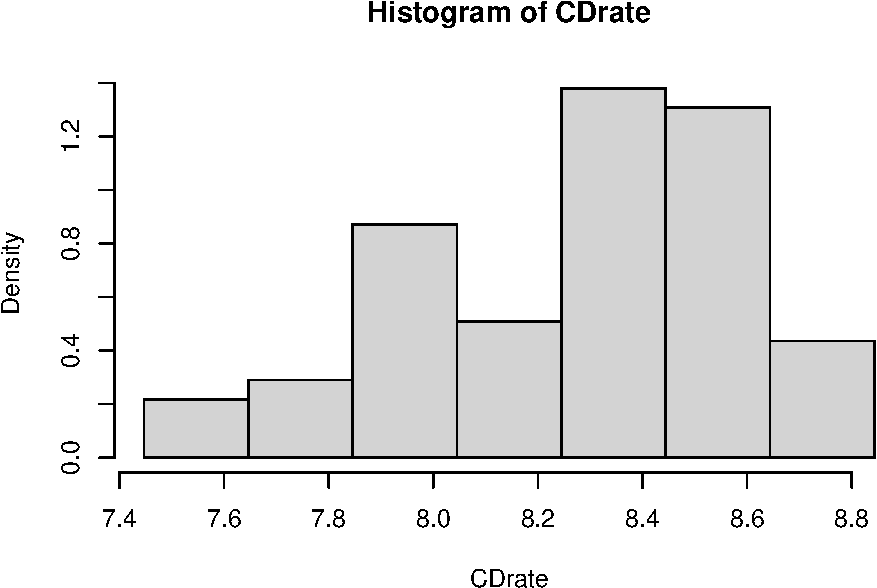
\includegraphics{20250930_AMA_Density_Estimation_files/figure-latex/2_Plot_hist-1} \end{center}

The following sentence converts this histogram into a function that can
be evaluated at any point of \(\mathbb{R}\), or at a vector of real
numbers:

\begin{Shaded}
\begin{Highlighting}[]
\NormalTok{hx\_f }\OtherTok{\textless{}{-}} \FunctionTok{stepfun}\NormalTok{(hx}\SpecialCharTok{$}\NormalTok{breaks, }\FunctionTok{c}\NormalTok{(}\DecValTok{0}\NormalTok{, hx}\SpecialCharTok{$}\NormalTok{density, }\DecValTok{0}\NormalTok{))}
\end{Highlighting}
\end{Shaded}

Use \texttt{hx\_f} to evaluate the histogram at the vector of observed
data \(x\). Then add the points \((x_i,\hat{f}_{\mathrm{hist}}(x_i))\),
\(i=1,\dots,n\), to the histogram you have plotted before.

\begin{Shaded}
\begin{Highlighting}[]
\CommentTok{\# Evaluate the histogram estimator at each data point}
\NormalTok{f\_hat }\OtherTok{\textless{}{-}} \FunctionTok{hx\_f}\NormalTok{(x)}

\CommentTok{\# Add the points to the plot}
\FunctionTok{plot}\NormalTok{(hx, }\AttributeTok{freq =} \ConstantTok{FALSE}\NormalTok{, }\AttributeTok{main =} \StringTok{"Histogram of CDrate"}\NormalTok{, }\AttributeTok{xlab =} \StringTok{"CDrate"}\NormalTok{)}
\FunctionTok{points}\NormalTok{(x, f\_hat, }\AttributeTok{col =} \StringTok{"blue"}\NormalTok{, }\AttributeTok{pch =} \DecValTok{19}\NormalTok{, }\AttributeTok{cex =} \FloatTok{0.5}\NormalTok{)}
\FunctionTok{legend}\NormalTok{(}\AttributeTok{x =} \FloatTok{7.5}\NormalTok{, }\AttributeTok{y =} \FloatTok{1.3}\NormalTok{, }\StringTok{"f\_hat(x\_i)"}\NormalTok{, }\AttributeTok{col =} \StringTok{"blue"}\NormalTok{, }\AttributeTok{pch =} \DecValTok{19}\NormalTok{)}
\end{Highlighting}
\end{Shaded}

\begin{center}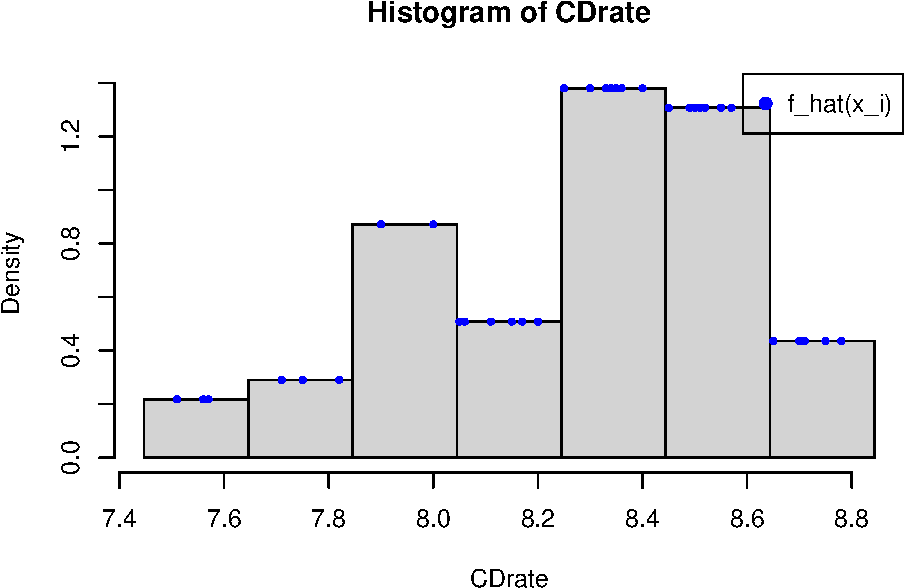
\includegraphics{20250930_AMA_Density_Estimation_files/figure-latex/plot_points_full-1} \end{center}

\begin{center}\rule{0.5\linewidth}{0.5pt}\end{center}

\subsection{3.}\label{section-2}

Use the formula you have found before relating
\(\hat{f}_{\mathrm{hist}}(x_i)\) and
\(\hat{f}_{\mathrm{hist},(-i)}(x_i)\) to compute
\(\hat{f}_{\mathrm{hist},(-i)}(x_i)\), \(i=1, \dots, n\). Then add the
points \((x_i,\hat{f}_{\mathrm{hist},(-i)}(x_i))\), \(i=1,\dots,n\), to
the previous plot.

\begin{Shaded}
\begin{Highlighting}[]
\CommentTok{\# Calculate bin width}
\NormalTok{b }\OtherTok{\textless{}{-}}\NormalTok{ (Z }\SpecialCharTok{{-}}\NormalTok{ A) }\SpecialCharTok{/}\NormalTok{ nbr}
\NormalTok{n }\OtherTok{\textless{}{-}} \FunctionTok{length}\NormalTok{(x)}

\CommentTok{\# Calculate the leave{-}one{-}out estimates}
\NormalTok{f\_loo }\OtherTok{\textless{}{-}}\NormalTok{ (n }\SpecialCharTok{/}\NormalTok{ (n }\SpecialCharTok{{-}} \DecValTok{1}\NormalTok{)) }\SpecialCharTok{*}\NormalTok{ f\_hat }\SpecialCharTok{{-}} \DecValTok{1} \SpecialCharTok{/}\NormalTok{ ((n }\SpecialCharTok{{-}} \DecValTok{1}\NormalTok{) }\SpecialCharTok{*}\NormalTok{ b)}

\CommentTok{\# Add the points to the plot}
\FunctionTok{plot}\NormalTok{(hx, }\AttributeTok{freq =} \ConstantTok{FALSE}\NormalTok{, }\AttributeTok{main =} \StringTok{"Histogram with Full and LOO Densities"}\NormalTok{, }\AttributeTok{xlab =} \StringTok{"CDrate"}\NormalTok{)}
\FunctionTok{points}\NormalTok{(x, f\_hat, }\AttributeTok{col =} \StringTok{"blue"}\NormalTok{, }\AttributeTok{pch =} \DecValTok{19}\NormalTok{, }\AttributeTok{cex =} \FloatTok{0.5}\NormalTok{)}
\FunctionTok{points}\NormalTok{(x, f\_loo, }\AttributeTok{col =} \StringTok{"red"}\NormalTok{, }\AttributeTok{pch =} \DecValTok{4}\NormalTok{, }\AttributeTok{cex =} \FloatTok{0.5}\NormalTok{)}
\FunctionTok{legend}\NormalTok{(}\AttributeTok{x =} \FloatTok{7.5}\NormalTok{, }\AttributeTok{y =} \FloatTok{1.3}\NormalTok{, }\FunctionTok{c}\NormalTok{(}\StringTok{"f\_hat(x\_i)"}\NormalTok{, }\StringTok{"f\_loo(x\_i)"}\NormalTok{), }\AttributeTok{col =} \FunctionTok{c}\NormalTok{(}\StringTok{"blue"}\NormalTok{, }\StringTok{"red"}\NormalTok{), }\AttributeTok{pch =} \FunctionTok{c}\NormalTok{(}\DecValTok{19}\NormalTok{, }\DecValTok{4}\NormalTok{))}
\end{Highlighting}
\end{Shaded}

\begin{center}\includegraphics{20250930_AMA_Density_Estimation_files/figure-latex/plot_points_loo-1} \end{center}

The blue dots show the histogram estimator of the density function for
each data point using the full dataset. As you can see, all dots within
the same bin are at the same height, being the top of that bin's bar.

The red crosses show the histogram estimator of the density function for
each data point if that point had been excluded from the calculation.

The red crosses are always slightly lower than the blue dots. Because
when we ``leave out'' a data point \(x_i\), the count of points in its
bin \(N_k\) decreases by one. Since the density is calculated as (count
/ total), reducing the count naturally leads to a lower density estimate
for that bin.

\begin{center}\rule{0.5\linewidth}{0.5pt}\end{center}

\subsection{4.}\label{section-3}

Compute the leave-one-out log-likelihood function corresponding to the
previous histogram, at which \texttt{nbr=7} has been used.

\begin{Shaded}
\begin{Highlighting}[]
\CommentTok{\# We only take the log of positive values. If f\_loo is 0, log(f\_loo) is {-}Inf.}
\CommentTok{\# This happens when a point is the only one in its bin.}
\NormalTok{looCV\_log\_lik\_7 }\OtherTok{\textless{}{-}} \FunctionTok{sum}\NormalTok{(}\FunctionTok{log}\NormalTok{(f\_loo[f\_loo }\SpecialCharTok{\textgreater{}} \DecValTok{0}\NormalTok{]))}
\FunctionTok{cat}\NormalTok{(}\StringTok{"Leave{-}one{-}out log{-}likelihood for nbr=7:"}\NormalTok{, looCV\_log\_lik\_7)}
\end{Highlighting}
\end{Shaded}

\begin{verbatim}
## Leave-one-out log-likelihood for nbr=7: -16.58432
\end{verbatim}

\textcolor{red}{Feedback and correction: This is wrong: $looCV_log_lik_nbr[i] <- sum(log(f_loo[f_loo > 0]))$ When selecting $[f_loo > 0]$you avoid vaues of the log-likelihood equal to -infinity. Nevertheless, a -infinity in the log-likelihood function has a clear meaning: your parameter choice is impossible! So you must not try to avoid -infinity values. It should be better to write $looCV_log_lik_nbr[i] <- sum(log(f_loo))$.}

\textcolor{red}{This correction will be made in question 4, 5, 6 and 7}

\textcolor{red}{After correction, we observe the same result as before meaning that all our values are positives and that our model will be able to make possible prediction for every points.}

\textcolor{red}{It's better to keep all values because a zero prediction (f_loo = 0) means the model considered that data point impossible. Including these zeros results in a log-likelihood of negative infinity, which correctly penalizes and disqualifies a model that makes impossible predictions.}

\begin{Shaded}
\begin{Highlighting}[]
\CommentTok{\# We take the log of all values.}
\NormalTok{looCV\_log\_lik\_7 }\OtherTok{\textless{}{-}} \FunctionTok{sum}\NormalTok{(}\FunctionTok{log}\NormalTok{(f\_loo))}
\FunctionTok{cat}\NormalTok{(}\StringTok{"Leave{-}one{-}out log{-}likelihood for nbr=7:"}\NormalTok{, looCV\_log\_lik\_7)}
\end{Highlighting}
\end{Shaded}

\begin{verbatim}
## Leave-one-out log-likelihood for nbr=7: -16.58432
\end{verbatim}

\begin{center}\rule{0.5\linewidth}{0.5pt}\end{center}

\subsection{5.}\label{section-4}

Consider now the set \texttt{seq(1,15)} as possible values for
\texttt{nbr}, the number of intervals of the histogram. For each of them
compute the leave-one-out log-likelihood function
(\texttt{looCV\_log\_lik}) for the corresponding histogram.

\begin{Shaded}
\begin{Highlighting}[]
\NormalTok{n }\OtherTok{\textless{}{-}} \FunctionTok{length}\NormalTok{(x)}
\NormalTok{nbr\_values }\OtherTok{\textless{}{-}} \DecValTok{1}\SpecialCharTok{:}\DecValTok{15}
\NormalTok{looCV\_log\_lik\_nbr }\OtherTok{\textless{}{-}} \FunctionTok{numeric}\NormalTok{(}\FunctionTok{length}\NormalTok{(nbr\_values))}

\ControlFlowTok{for}\NormalTok{ (i }\ControlFlowTok{in} \FunctionTok{seq\_along}\NormalTok{(nbr\_values)) \{}
\NormalTok{  current\_nbr }\OtherTok{\textless{}{-}}\NormalTok{ nbr\_values[i]}
\NormalTok{  b }\OtherTok{\textless{}{-}}\NormalTok{ (Z }\SpecialCharTok{{-}}\NormalTok{ A) }\SpecialCharTok{/}\NormalTok{ current\_nbr}
  
  \CommentTok{\# Create histogram object}
\NormalTok{  hx }\OtherTok{\textless{}{-}} \FunctionTok{hist}\NormalTok{(x, }\AttributeTok{breaks =} \FunctionTok{seq}\NormalTok{(A, Z, }\AttributeTok{length =}\NormalTok{ current\_nbr }\SpecialCharTok{+} \DecValTok{1}\NormalTok{), }\AttributeTok{plot =} \ConstantTok{FALSE}\NormalTok{)}
  
  \CommentTok{\# Create step function}
\NormalTok{  hx\_f }\OtherTok{\textless{}{-}} \FunctionTok{stepfun}\NormalTok{(hx}\SpecialCharTok{$}\NormalTok{breaks, }\FunctionTok{c}\NormalTok{(}\DecValTok{0}\NormalTok{, hx}\SpecialCharTok{$}\NormalTok{density, }\DecValTok{0}\NormalTok{))}
  
  \CommentTok{\# Calculate f\_hat and f\_loo}
\NormalTok{  f\_hat }\OtherTok{\textless{}{-}} \FunctionTok{hx\_f}\NormalTok{(x)}
\NormalTok{  f\_loo }\OtherTok{\textless{}{-}}\NormalTok{ (n }\SpecialCharTok{/}\NormalTok{ (n }\SpecialCharTok{{-}} \DecValTok{1}\NormalTok{)) }\SpecialCharTok{*}\NormalTok{ f\_hat }\SpecialCharTok{{-}} \DecValTok{1} \SpecialCharTok{/}\NormalTok{ ((n }\SpecialCharTok{{-}} \DecValTok{1}\NormalTok{) }\SpecialCharTok{*}\NormalTok{ b)}
  
  \CommentTok{\# Calculate and store looCV log{-}likelihood}
\NormalTok{  looCV\_log\_lik\_nbr[i] }\OtherTok{\textless{}{-}} \FunctionTok{sum}\NormalTok{(}\FunctionTok{log}\NormalTok{(f\_loo))}
\NormalTok{\}}

\CommentTok{\# Plot the results}
\FunctionTok{plot}\NormalTok{(nbr\_values, looCV\_log\_lik\_nbr, }\AttributeTok{type =} \StringTok{"b"}\NormalTok{, }\AttributeTok{pch =} \DecValTok{19}\NormalTok{,}
     \AttributeTok{xlab =} \StringTok{"Number of Bins (nbr)"}\NormalTok{, }\AttributeTok{ylab =} \StringTok{"LOO Log{-}Likelihood"}\NormalTok{,}
     \AttributeTok{main =} \StringTok{"LOO Cross{-}Validation for Number of Bins"}\NormalTok{)}

\CommentTok{\# Find the optimal nbr}
\NormalTok{optimal\_nbr }\OtherTok{\textless{}{-}}\NormalTok{ nbr\_values[}\FunctionTok{which.max}\NormalTok{(looCV\_log\_lik\_nbr)]}
\FunctionTok{abline}\NormalTok{(}\AttributeTok{v =}\NormalTok{ optimal\_nbr, }\AttributeTok{col =} \StringTok{"red"}\NormalTok{, }\AttributeTok{lty =} \DecValTok{2}\NormalTok{)}
\FunctionTok{legend}\NormalTok{(}\StringTok{"bottomleft"}\NormalTok{, }\AttributeTok{legend =} \FunctionTok{paste}\NormalTok{(}\StringTok{"Optimal nbr ="}\NormalTok{, optimal\_nbr), }\AttributeTok{col =} \StringTok{"red"}\NormalTok{, }\AttributeTok{lty =} \DecValTok{2}\NormalTok{)}
\end{Highlighting}
\end{Shaded}

\begin{center}\includegraphics{20250930_AMA_Density_Estimation_files/figure-latex/nbr_loocv-1} \end{center}

The plot displays the leave-one-out log-likelihood score for histograms
with a varying number of bins (nbr). The score increases to a distinct
peak at nbr = 5, which is the value that maximizes the log-likelihood.
After this point, the performance becomes more erratic and generally
decreases.

Therefore, according to the looCV method, the optimal choice for the
number of bins is 5 for this dataset. Unlike the previous analysis,
there is a clear peak, and choosing a higher nbr would likely result in
overfitting.

Finally, plot the histogram of \(x\) using the optimal value of
\texttt{nbr}.

\begin{Shaded}
\begin{Highlighting}[]
\FunctionTok{hist}\NormalTok{(x, }\AttributeTok{breaks =} \FunctionTok{seq}\NormalTok{(A, Z, }\AttributeTok{length =}\NormalTok{ optimal\_nbr }\SpecialCharTok{+} \DecValTok{1}\NormalTok{), }\AttributeTok{freq =} \ConstantTok{FALSE}\NormalTok{,}
     \AttributeTok{main =} \FunctionTok{paste}\NormalTok{(}\StringTok{"Optimal Histogram (nbr ="}\NormalTok{, optimal\_nbr, }\StringTok{")"}\NormalTok{),}
     \AttributeTok{xlab =} \StringTok{"CDrate"}\NormalTok{)}
\end{Highlighting}
\end{Shaded}

\begin{center}\includegraphics{20250930_AMA_Density_Estimation_files/figure-latex/plot_optimal_nbr-1} \end{center}

\begin{center}\rule{0.5\linewidth}{0.5pt}\end{center}

\subsection{6.}\label{section-5}

Let \texttt{b} be the common width of the bins of a histogram. Consider
the set \texttt{seq((Z-A)/15,(Z-A)/1,length=30)} as possible values for
\texttt{b}. Select the value of \texttt{b} maximizing the leave-one-out
log-likelihood function, and plot the corresponding histogram.

\begin{Shaded}
\begin{Highlighting}[]
\NormalTok{b\_values }\OtherTok{\textless{}{-}} \FunctionTok{seq}\NormalTok{((Z }\SpecialCharTok{{-}}\NormalTok{ A) }\SpecialCharTok{/} \DecValTok{15}\NormalTok{, (Z }\SpecialCharTok{{-}}\NormalTok{ A) }\SpecialCharTok{/} \DecValTok{1}\NormalTok{, }\AttributeTok{length =} \DecValTok{30}\NormalTok{)}
\NormalTok{looCV\_log\_lik\_b }\OtherTok{\textless{}{-}} \FunctionTok{numeric}\NormalTok{(}\FunctionTok{length}\NormalTok{(b\_values))}

\ControlFlowTok{for}\NormalTok{ (i }\ControlFlowTok{in} \FunctionTok{seq\_along}\NormalTok{(b\_values)) \{}
\NormalTok{  current\_b }\OtherTok{\textless{}{-}}\NormalTok{ b\_values[i]}
  
  \CommentTok{\# Create histogram object with specified bin width}
\NormalTok{  hx }\OtherTok{\textless{}{-}} \FunctionTok{hist}\NormalTok{(x, }\AttributeTok{breaks =} \FunctionTok{seq}\NormalTok{(A, Z }\SpecialCharTok{+}\NormalTok{ current\_b, }\AttributeTok{by =}\NormalTok{ current\_b), }\AttributeTok{plot =} \ConstantTok{FALSE}\NormalTok{)}
  
  \CommentTok{\# Create step function}
\NormalTok{  hx\_f }\OtherTok{\textless{}{-}} \FunctionTok{stepfun}\NormalTok{(hx}\SpecialCharTok{$}\NormalTok{breaks, }\FunctionTok{c}\NormalTok{(}\DecValTok{0}\NormalTok{, hx}\SpecialCharTok{$}\NormalTok{density, }\DecValTok{0}\NormalTok{))}
  
  \CommentTok{\# Calculate f\_hat and f\_loo}
\NormalTok{  f\_hat }\OtherTok{\textless{}{-}} \FunctionTok{hx\_f}\NormalTok{(x)}
\NormalTok{  f\_loo }\OtherTok{\textless{}{-}}\NormalTok{ (n }\SpecialCharTok{/}\NormalTok{ (n }\SpecialCharTok{{-}} \DecValTok{1}\NormalTok{)) }\SpecialCharTok{*}\NormalTok{ f\_hat }\SpecialCharTok{{-}} \DecValTok{1} \SpecialCharTok{/}\NormalTok{ ((n }\SpecialCharTok{{-}} \DecValTok{1}\NormalTok{) }\SpecialCharTok{*}\NormalTok{ current\_b)}
  
  \CommentTok{\# Calculate and store looCV log{-}likelihood}
\NormalTok{  looCV\_log\_lik\_b[i] }\OtherTok{\textless{}{-}} \FunctionTok{sum}\NormalTok{(}\FunctionTok{log}\NormalTok{(f\_loo))}
\NormalTok{\}}

\CommentTok{\# Plot the results}
\FunctionTok{plot}\NormalTok{(b\_values, looCV\_log\_lik\_b, }\AttributeTok{type =} \StringTok{"b"}\NormalTok{, }\AttributeTok{pch =} \DecValTok{19}\NormalTok{,}
     \AttributeTok{xlab =} \StringTok{"Bin Width (b)"}\NormalTok{, }\AttributeTok{ylab =} \StringTok{"LOO Log{-}Likelihood"}\NormalTok{,}
     \AttributeTok{main =} \StringTok{"LOO Cross{-}Validation for Bin Width"}\NormalTok{)}

\CommentTok{\# Find the optimal b}
\NormalTok{optimal\_b }\OtherTok{\textless{}{-}}\NormalTok{ b\_values[}\FunctionTok{which.max}\NormalTok{(looCV\_log\_lik\_b)]}
\FunctionTok{abline}\NormalTok{(}\AttributeTok{v =}\NormalTok{ optimal\_b, }\AttributeTok{col =} \StringTok{"red"}\NormalTok{, }\AttributeTok{lty =} \DecValTok{2}\NormalTok{)}
\FunctionTok{legend}\NormalTok{(}\StringTok{"topright"}\NormalTok{, }\AttributeTok{legend =} \FunctionTok{paste}\NormalTok{(}\StringTok{"Optimal b ="}\NormalTok{, }\FunctionTok{round}\NormalTok{(optimal\_b, }\DecValTok{3}\NormalTok{)), }\AttributeTok{col =} \StringTok{"red"}\NormalTok{, }\AttributeTok{lty =} \DecValTok{2}\NormalTok{)}
\end{Highlighting}
\end{Shaded}

\begin{center}\includegraphics{20250930_AMA_Density_Estimation_files/figure-latex/b_loocv-1} \end{center}

Plot the corresponding histogram.

\begin{Shaded}
\begin{Highlighting}[]
\NormalTok{hx\_optimal\_b }\OtherTok{\textless{}{-}} \FunctionTok{hist}\NormalTok{(x, }\AttributeTok{breaks =} \FunctionTok{seq}\NormalTok{(A, Z }\SpecialCharTok{+}\NormalTok{ optimal\_b, }\AttributeTok{by =}\NormalTok{ optimal\_b), }\AttributeTok{plot =} \ConstantTok{FALSE}\NormalTok{)}
\FunctionTok{plot}\NormalTok{(hx\_optimal\_b, }\AttributeTok{freq =} \ConstantTok{FALSE}\NormalTok{,}
     \AttributeTok{main =} \FunctionTok{paste}\NormalTok{(}\StringTok{"Optimal Histogram (b ="}\NormalTok{, }\FunctionTok{round}\NormalTok{(optimal\_b, }\DecValTok{3}\NormalTok{), }\StringTok{")"}\NormalTok{),}
     \AttributeTok{xlab =} \StringTok{"CDrate"}\NormalTok{)}
\end{Highlighting}
\end{Shaded}

\begin{center}\includegraphics{20250930_AMA_Density_Estimation_files/figure-latex/plot_optimal_b-1} \end{center}

\textcolor{red}{As we can see from the new plots after correction, both optimization methods—choosing the number of bins (nbr) and choosing the bin width (b) directly—converge on the same optimal histogram structure. The analysis for nbr found that 5 bins were optimal, and the analysis for b found an optimal width of 0.273, which also results in a 5-bin histogram. This confirms that the model with 5 bins provides the most robust predictive fit for this dataset.}

\begin{center}\rule{0.5\linewidth}{0.5pt}\end{center}

\subsection{7.}\label{section-6}

Recycle the functions \texttt{graph.mixt} and \texttt{sim.mixt} to
generate \(n=100\) data from
\[ f(x) = (3/4)N(x; m = 0, s = 1) +(1/4) N(x; m = 3/2, s = 1/3) \]

\begin{Shaded}
\begin{Highlighting}[]
\CommentTok{\# Generate 100 observations from f(x) = (3/4)N(x; m = 0, s = 1) +(1/4) N(x; m = 3/2, s = 1/3)}
\FunctionTok{set.seed}\NormalTok{(}\DecValTok{123}\NormalTok{)}
\NormalTok{n }\OtherTok{\textless{}{-}} \DecValTok{100}
\NormalTok{mu }\OtherTok{\textless{}{-}} \FunctionTok{c}\NormalTok{(}\DecValTok{0}\NormalTok{,}\DecValTok{3}\SpecialCharTok{/}\DecValTok{2}\NormalTok{)}
\NormalTok{sigma }\OtherTok{\textless{}{-}} \FunctionTok{c}\NormalTok{(}\DecValTok{1}\NormalTok{,}\DecValTok{1}\SpecialCharTok{/}\DecValTok{3}\NormalTok{)}
\NormalTok{alpha }\OtherTok{\textless{}{-}} \FunctionTok{c}\NormalTok{(}\DecValTok{3}\SpecialCharTok{/}\DecValTok{4}\NormalTok{,}\DecValTok{1}\SpecialCharTok{/}\DecValTok{4}\NormalTok{)}
\NormalTok{x }\OtherTok{\textless{}{-}} \FunctionTok{sim.mixt}\NormalTok{(}\AttributeTok{n=}\NormalTok{n, }\AttributeTok{k=}\DecValTok{2}\NormalTok{, }\AttributeTok{mu=}\NormalTok{mu, }\AttributeTok{sigma=}\NormalTok{sigma, }\AttributeTok{alpha=}\NormalTok{alpha)}
\NormalTok{f\_x }\OtherTok{\textless{}{-}} \FunctionTok{graph.mixt}\NormalTok{(}\AttributeTok{k=}\DecValTok{2}\NormalTok{, }\AttributeTok{mu=}\NormalTok{mu, }\AttributeTok{sigma=}\NormalTok{sigma, }\AttributeTok{alpha=}\NormalTok{alpha, }\AttributeTok{graphic =}\NormalTok{ F)}
\end{Highlighting}
\end{Shaded}

Let \(b\) be the bin width of a histogram estimator of \(f(x)\) using
the generated data. Select the value of \(b\) maximizing the
leave-one-out log-likelihood function, and plot the corresponding
histogram.

\begin{Shaded}
\begin{Highlighting}[]
\CommentTok{\#We will use the same method as before}
\NormalTok{A }\OtherTok{\textless{}{-}} \FunctionTok{min}\NormalTok{(x) }\SpecialCharTok{{-}} \FloatTok{0.05} \SpecialCharTok{*} \FunctionTok{diff}\NormalTok{(}\FunctionTok{range}\NormalTok{(x))}
\NormalTok{Z }\OtherTok{\textless{}{-}} \FunctionTok{max}\NormalTok{(x) }\SpecialCharTok{+} \FloatTok{0.05} \SpecialCharTok{*} \FunctionTok{diff}\NormalTok{(}\FunctionTok{range}\NormalTok{(x))}

\NormalTok{b\_values }\OtherTok{\textless{}{-}} \FunctionTok{seq}\NormalTok{((Z }\SpecialCharTok{{-}}\NormalTok{ A) }\SpecialCharTok{/} \DecValTok{15}\NormalTok{, (Z }\SpecialCharTok{{-}}\NormalTok{ A) }\SpecialCharTok{/} \DecValTok{1}\NormalTok{, }\AttributeTok{length =} \DecValTok{30}\NormalTok{)}
\NormalTok{looCV\_log\_lik\_b }\OtherTok{\textless{}{-}} \FunctionTok{numeric}\NormalTok{(}\FunctionTok{length}\NormalTok{(b\_values))}

\ControlFlowTok{for}\NormalTok{ (i }\ControlFlowTok{in} \FunctionTok{seq\_along}\NormalTok{(b\_values)) \{}
\NormalTok{  current\_b }\OtherTok{\textless{}{-}}\NormalTok{ b\_values[i]}
  
  \CommentTok{\# Create histogram object with specified bin width}
\NormalTok{  hx }\OtherTok{\textless{}{-}} \FunctionTok{hist}\NormalTok{(x, }\AttributeTok{breaks =} \FunctionTok{seq}\NormalTok{(A, Z }\SpecialCharTok{+}\NormalTok{ current\_b, }\AttributeTok{by =}\NormalTok{ current\_b), }\AttributeTok{plot =} \ConstantTok{FALSE}\NormalTok{)}
  
  \CommentTok{\# Create step function}
\NormalTok{  hx\_f }\OtherTok{\textless{}{-}} \FunctionTok{stepfun}\NormalTok{(hx}\SpecialCharTok{$}\NormalTok{breaks, }\FunctionTok{c}\NormalTok{(}\DecValTok{0}\NormalTok{, hx}\SpecialCharTok{$}\NormalTok{density, }\DecValTok{0}\NormalTok{))}
  
  \CommentTok{\# Calculate f\_hat and f\_loo}
\NormalTok{  f\_hat }\OtherTok{\textless{}{-}} \FunctionTok{hx\_f}\NormalTok{(x)}
\NormalTok{  f\_loo }\OtherTok{\textless{}{-}}\NormalTok{ (n }\SpecialCharTok{/}\NormalTok{ (n }\SpecialCharTok{{-}} \DecValTok{1}\NormalTok{)) }\SpecialCharTok{*}\NormalTok{ f\_hat }\SpecialCharTok{{-}} \DecValTok{1} \SpecialCharTok{/}\NormalTok{ ((n }\SpecialCharTok{{-}} \DecValTok{1}\NormalTok{) }\SpecialCharTok{*}\NormalTok{ current\_b)}
  
  \CommentTok{\# Calculate and store looCV log{-}likelihood}
\NormalTok{  looCV\_log\_lik\_b[i] }\OtherTok{\textless{}{-}} \FunctionTok{sum}\NormalTok{(}\FunctionTok{log}\NormalTok{(f\_loo))}
\NormalTok{\}}

\CommentTok{\# Plot the results}
\FunctionTok{plot}\NormalTok{(b\_values, looCV\_log\_lik\_b, }\AttributeTok{type =} \StringTok{"b"}\NormalTok{, }\AttributeTok{pch =} \DecValTok{19}\NormalTok{,}
     \AttributeTok{xlab =} \StringTok{"Bin Width (b)"}\NormalTok{, }\AttributeTok{ylab =} \StringTok{"LOO Log{-}Likelihood"}\NormalTok{,}
     \AttributeTok{main =} \StringTok{"LOO Cross{-}Validation for Bin Width"}\NormalTok{)}

\CommentTok{\# Find the optimal b}
\NormalTok{optimal\_b }\OtherTok{\textless{}{-}}\NormalTok{ b\_values[}\FunctionTok{which.max}\NormalTok{(looCV\_log\_lik\_b)]}
\FunctionTok{abline}\NormalTok{(}\AttributeTok{v =}\NormalTok{ optimal\_b, }\AttributeTok{col =} \StringTok{"red"}\NormalTok{, }\AttributeTok{lty =} \DecValTok{2}\NormalTok{)}
\FunctionTok{legend}\NormalTok{(}\StringTok{"topright"}\NormalTok{, }\AttributeTok{legend =} \FunctionTok{paste}\NormalTok{(}\StringTok{"Optimal b ="}\NormalTok{, }\FunctionTok{round}\NormalTok{(optimal\_b, }\DecValTok{3}\NormalTok{)), }\AttributeTok{col =} \StringTok{"red"}\NormalTok{, }\AttributeTok{lty =} \DecValTok{2}\NormalTok{)}
\end{Highlighting}
\end{Shaded}

\begin{center}\includegraphics{20250930_AMA_Density_Estimation_files/figure-latex/max_sim_mixt-1} \end{center}

\begin{Shaded}
\begin{Highlighting}[]
\NormalTok{hx\_optimal\_b }\OtherTok{\textless{}{-}} \FunctionTok{hist}\NormalTok{(x, }\AttributeTok{breaks =} \FunctionTok{seq}\NormalTok{(A, Z }\SpecialCharTok{+}\NormalTok{ optimal\_b, }\AttributeTok{by =}\NormalTok{ optimal\_b), }\AttributeTok{plot =} \ConstantTok{FALSE}\NormalTok{)}
\FunctionTok{plot}\NormalTok{(hx\_optimal\_b, }\AttributeTok{freq =} \ConstantTok{FALSE}\NormalTok{,}
     \AttributeTok{main =} \FunctionTok{paste}\NormalTok{(}\StringTok{"Optimal Histogram (b ="}\NormalTok{, }\FunctionTok{round}\NormalTok{(optimal\_b, }\DecValTok{3}\NormalTok{), }\StringTok{")"}\NormalTok{),}
     \AttributeTok{xlab =} \StringTok{"CDrate"}\NormalTok{)}
\FunctionTok{lines}\NormalTok{(f\_x}\SpecialCharTok{$}\NormalTok{x, f\_x}\SpecialCharTok{$}\NormalTok{fx, }\AttributeTok{lwd =} \DecValTok{2}\NormalTok{)}
\end{Highlighting}
\end{Shaded}

\begin{center}\includegraphics{20250930_AMA_Density_Estimation_files/figure-latex/hist_opt_sim_mixt-1} \end{center}

Compare with the results obtained using the Scott's formula:

\[ b_{Scott}=3.49St.Dev(X)n^{-1/3} \]

\begin{Shaded}
\begin{Highlighting}[]
\NormalTok{scott\_b }\OtherTok{\textless{}{-}} \FloatTok{3.49} \SpecialCharTok{*} \FunctionTok{sd}\NormalTok{(x) }\SpecialCharTok{*}\NormalTok{ (}\FunctionTok{length}\NormalTok{(x)}\SpecialCharTok{\^{}}\NormalTok{(}\SpecialCharTok{{-}}\DecValTok{1}\SpecialCharTok{/}\DecValTok{3}\NormalTok{))}
\NormalTok{hx\_scott\_b }\OtherTok{\textless{}{-}} \FunctionTok{hist}\NormalTok{(x, }\AttributeTok{breaks =} \FunctionTok{seq}\NormalTok{(A, Z }\SpecialCharTok{+}\NormalTok{ scott\_b, }\AttributeTok{by =}\NormalTok{ scott\_b), }\AttributeTok{plot =} \ConstantTok{FALSE}\NormalTok{)}
\NormalTok{ymax }\OtherTok{\textless{}{-}} \FunctionTok{max}\NormalTok{(}\FunctionTok{c}\NormalTok{(hx\_scott\_b}\SpecialCharTok{$}\NormalTok{y, f\_x}\SpecialCharTok{$}\NormalTok{fx))}
\FunctionTok{plot}\NormalTok{(hx\_scott\_b, }\AttributeTok{freq =} \ConstantTok{FALSE}\NormalTok{, }\AttributeTok{ylim =} \FunctionTok{c}\NormalTok{(}\DecValTok{0}\NormalTok{, ymax),}
     \AttributeTok{main =} \FunctionTok{paste}\NormalTok{(}\StringTok{"Optimal Histogram (b\_scott ="}\NormalTok{, }\FunctionTok{round}\NormalTok{(scott\_b, }\DecValTok{3}\NormalTok{), }\StringTok{")"}\NormalTok{),}
     \AttributeTok{xlab =} \StringTok{"CDrate"}\NormalTok{)}
\FunctionTok{lines}\NormalTok{(f\_x}\SpecialCharTok{$}\NormalTok{x, f\_x}\SpecialCharTok{$}\NormalTok{fx, }\AttributeTok{lwd =} \DecValTok{2}\NormalTok{)}
\end{Highlighting}
\end{Shaded}

\begin{center}\includegraphics{20250930_AMA_Density_Estimation_files/figure-latex/hist_scott-1} \end{center}

In this case, the \(b\) that maximized the leave-one-out log-likelihood
provided a better fit than Scott's formula for choosing \(b\). This can
be proved by calculating the MSE of the estimators.

\begin{Shaded}
\begin{Highlighting}[]
\CommentTok{\# Compute histogram densities as step functions}
\NormalTok{hx\_scott\_f }\OtherTok{\textless{}{-}} \FunctionTok{stepfun}\NormalTok{(hx\_scott\_b}\SpecialCharTok{$}\NormalTok{breaks, }\FunctionTok{c}\NormalTok{(}\DecValTok{0}\NormalTok{, hx\_scott\_b}\SpecialCharTok{$}\NormalTok{density, }\DecValTok{0}\NormalTok{))}
\NormalTok{hx\_optimal\_f }\OtherTok{\textless{}{-}} \FunctionTok{stepfun}\NormalTok{(hx\_optimal\_b}\SpecialCharTok{$}\NormalTok{breaks, }\FunctionTok{c}\NormalTok{(}\DecValTok{0}\NormalTok{, hx\_optimal\_b}\SpecialCharTok{$}\NormalTok{density, }\DecValTok{0}\NormalTok{))}

\CommentTok{\# Evaluate histogram estimates at the grid of f\_x}
\NormalTok{f\_hat\_scott }\OtherTok{\textless{}{-}} \FunctionTok{hx\_scott\_f}\NormalTok{(f\_x}\SpecialCharTok{$}\NormalTok{x)}
\NormalTok{f\_hat\_optimal }\OtherTok{\textless{}{-}} \FunctionTok{hx\_optimal\_f}\NormalTok{(f\_x}\SpecialCharTok{$}\NormalTok{x)}

\CommentTok{\# Compute MSE for Scott\textquotesingle{}s rule and Optimal b}
\NormalTok{mse\_scott }\OtherTok{\textless{}{-}} \FunctionTok{mean}\NormalTok{((f\_hat\_scott }\SpecialCharTok{{-}}\NormalTok{ f\_x}\SpecialCharTok{$}\NormalTok{fx)}\SpecialCharTok{\^{}}\DecValTok{2}\NormalTok{)}
\NormalTok{mse\_optimal }\OtherTok{\textless{}{-}} \FunctionTok{mean}\NormalTok{((f\_hat\_optimal }\SpecialCharTok{{-}}\NormalTok{ f\_x}\SpecialCharTok{$}\NormalTok{fx)}\SpecialCharTok{\^{}}\DecValTok{2}\NormalTok{)}

\CommentTok{\# Print results}
\FunctionTok{cat}\NormalTok{(}\StringTok{"MSE (Scott\textquotesingle{}s rule):"}\NormalTok{, mse\_scott, }\StringTok{"}\SpecialCharTok{\textbackslash{}n}\StringTok{"}\NormalTok{)}
\end{Highlighting}
\end{Shaded}

\begin{verbatim}
## MSE (Scott's rule): 0.002943868
\end{verbatim}

\begin{Shaded}
\begin{Highlighting}[]
\FunctionTok{cat}\NormalTok{(}\StringTok{"MSE (Optimal b):"}\NormalTok{, mse\_optimal, }\StringTok{"}\SpecialCharTok{\textbackslash{}n}\StringTok{"}\NormalTok{)}
\end{Highlighting}
\end{Shaded}

\begin{verbatim}
## MSE (Optimal b): 0.00459882
\end{verbatim}

\section{Kernel Density Estimator}\label{kernel-density-estimator}

\subsection{8.}\label{section-7}

Consider the vector x of data you have generated before from the mixture
of two normal. Use the relationship

\[ \hat{f}_{h,(-i)}(x_i)=\frac{n}{n-1}\left(\hat{f}_h(x_i)-\frac{K(0)}{nh}\right) \]

to select the value of h maximizing the leave-one-out log-likelihood
function, and plot the corresponding kernel density estimator.

\begin{Shaded}
\begin{Highlighting}[]
\NormalTok{n }\OtherTok{\textless{}{-}} \FunctionTok{length}\NormalTok{(x)}
\NormalTok{K0 }\OtherTok{\textless{}{-}} \FunctionTok{dnorm}\NormalTok{(}\DecValTok{0}\NormalTok{)}

\NormalTok{kx0 }\OtherTok{\textless{}{-}} \FunctionTok{density}\NormalTok{(x) }
\NormalTok{base\_bw }\OtherTok{\textless{}{-}}\NormalTok{ kx0}\SpecialCharTok{$}\NormalTok{bw}
\NormalTok{h\_values }\OtherTok{\textless{}{-}} \FunctionTok{seq}\NormalTok{(base\_bw}\SpecialCharTok{/}\DecValTok{5}\NormalTok{, base\_bw}\SpecialCharTok{*}\DecValTok{3}\NormalTok{, }\AttributeTok{length.out =} \DecValTok{50}\NormalTok{)}

\NormalTok{loo\_loglik\_h }\OtherTok{\textless{}{-}} \FunctionTok{numeric}\NormalTok{(}\FunctionTok{length}\NormalTok{(h\_values))}

\ControlFlowTok{for}\NormalTok{ (i }\ControlFlowTok{in} \FunctionTok{seq\_along}\NormalTok{(h\_values)) \{}
\NormalTok{  h }\OtherTok{\textless{}{-}}\NormalTok{ h\_values[i]}
\NormalTok{  kx }\OtherTok{\textless{}{-}} \FunctionTok{density}\NormalTok{(x, }\AttributeTok{bw =}\NormalTok{ h, }\AttributeTok{kernel =} \StringTok{"gaussian"}\NormalTok{, }\AttributeTok{n =} \DecValTok{1024}\NormalTok{,}
                \AttributeTok{from =} \FunctionTok{min}\NormalTok{(x) }\SpecialCharTok{{-}} \DecValTok{3}\SpecialCharTok{*}\NormalTok{h, }\AttributeTok{to =} \FunctionTok{max}\NormalTok{(x) }\SpecialCharTok{+} \DecValTok{3}\SpecialCharTok{*}\NormalTok{h)}
\NormalTok{  kx\_f }\OtherTok{\textless{}{-}} \FunctionTok{approxfun}\NormalTok{(}\AttributeTok{x =}\NormalTok{ kx}\SpecialCharTok{$}\NormalTok{x, }\AttributeTok{y =}\NormalTok{ kx}\SpecialCharTok{$}\NormalTok{y, }\AttributeTok{rule =} \DecValTok{2}\NormalTok{)}
\NormalTok{  f\_hat }\OtherTok{\textless{}{-}} \FunctionTok{kx\_f}\NormalTok{(x)                      }\CommentTok{\# approx f\_hat at each xi}
\NormalTok{  f\_loo }\OtherTok{\textless{}{-}}\NormalTok{ (n }\SpecialCharTok{/}\NormalTok{ (n }\SpecialCharTok{{-}} \DecValTok{1}\NormalTok{)) }\SpecialCharTok{*}\NormalTok{ (f\_hat }\SpecialCharTok{{-}}\NormalTok{ K0 }\SpecialCharTok{/}\NormalTok{ (n }\SpecialCharTok{*}\NormalTok{ h))}
\NormalTok{  pos }\OtherTok{\textless{}{-}}\NormalTok{ f\_loo }\SpecialCharTok{\textgreater{}} \DecValTok{0}
  \ControlFlowTok{if}\NormalTok{ (}\FunctionTok{any}\NormalTok{(pos)) \{}
\NormalTok{    loo\_loglik\_h[i] }\OtherTok{\textless{}{-}} \FunctionTok{sum}\NormalTok{(}\FunctionTok{log}\NormalTok{(f\_loo[pos]))}
\NormalTok{  \} }\ControlFlowTok{else}\NormalTok{ \{}
\NormalTok{    loo\_loglik\_h[i] }\OtherTok{\textless{}{-}} \SpecialCharTok{{-}}\ConstantTok{Inf}
\NormalTok{  \}}
\NormalTok{\}}

\NormalTok{optimal\_h\_approx }\OtherTok{\textless{}{-}}\NormalTok{ h\_values[}\FunctionTok{which.max}\NormalTok{(loo\_loglik\_h)]}
\FunctionTok{cat}\NormalTok{(}\StringTok{"Optimal h (approx) ="}\NormalTok{, optimal\_h\_approx, }\StringTok{"}\SpecialCharTok{\textbackslash{}n}\StringTok{"}\NormalTok{)}
\end{Highlighting}
\end{Shaded}

\begin{verbatim}
## Optimal h (approx) = 0.3281848
\end{verbatim}

\begin{Shaded}
\begin{Highlighting}[]
\FunctionTok{plot}\NormalTok{(h\_values, loo\_loglik\_h, }\AttributeTok{type =} \StringTok{"b"}\NormalTok{, }\AttributeTok{pch =} \DecValTok{19}\NormalTok{,}
     \AttributeTok{xlab =} \StringTok{"Bandwidth (h)"}\NormalTok{, }\AttributeTok{ylab =} \StringTok{"LOO log{-}likelihood"}\NormalTok{,}
     \AttributeTok{main =} \StringTok{"LOO CV for KDE bandwidth (approx)"}\NormalTok{)}
\FunctionTok{abline}\NormalTok{(}\AttributeTok{v =}\NormalTok{ optimal\_h\_approx, }\AttributeTok{col =} \StringTok{"red"}\NormalTok{, }\AttributeTok{lty =} \DecValTok{2}\NormalTok{)}
\FunctionTok{legend}\NormalTok{(}\StringTok{"bottomright"}\NormalTok{, }\AttributeTok{legend =} \FunctionTok{paste}\NormalTok{(}\StringTok{"optimal h ="}\NormalTok{, }\FunctionTok{round}\NormalTok{(optimal\_h\_approx, }\DecValTok{4}\NormalTok{)),}
       \AttributeTok{col =} \StringTok{"red"}\NormalTok{, }\AttributeTok{lty =} \DecValTok{2}\NormalTok{)}
\end{Highlighting}
\end{Shaded}

\begin{center}\includegraphics{20250930_AMA_Density_Estimation_files/figure-latex/loo_KDE-1} \end{center}

\begin{Shaded}
\begin{Highlighting}[]
\NormalTok{kx\_opt }\OtherTok{\textless{}{-}} \FunctionTok{density}\NormalTok{(x, }\AttributeTok{bw =}\NormalTok{ optimal\_h\_approx, }\AttributeTok{kernel =} \StringTok{"gaussian"}\NormalTok{)}

\CommentTok{\# Common ylim so both functions fit inside the plot}
\NormalTok{ymax }\OtherTok{\textless{}{-}} \FunctionTok{max}\NormalTok{(}\FunctionTok{c}\NormalTok{(kx\_opt}\SpecialCharTok{$}\NormalTok{y, f\_x}\SpecialCharTok{$}\NormalTok{fx))}


\FunctionTok{plot}\NormalTok{(kx\_opt, }
     \AttributeTok{ylim =} \FunctionTok{c}\NormalTok{(}\DecValTok{0}\NormalTok{, ymax), }
     \AttributeTok{main =} \FunctionTok{paste}\NormalTok{(}\StringTok{"KDE (h ="}\NormalTok{, }\FunctionTok{round}\NormalTok{(optimal\_h\_approx, }\DecValTok{4}\NormalTok{), }\StringTok{")"}\NormalTok{), }
     \AttributeTok{col =} \StringTok{"blue"}\NormalTok{, }
     \AttributeTok{lwd =} \DecValTok{2}\NormalTok{)}

\FunctionTok{lines}\NormalTok{(f\_x}\SpecialCharTok{$}\NormalTok{x, f\_x}\SpecialCharTok{$}\NormalTok{fx, }\AttributeTok{col =} \StringTok{"black"}\NormalTok{, }\AttributeTok{lwd =} \DecValTok{2}\NormalTok{)}

\FunctionTok{legend}\NormalTok{(}\StringTok{"topright"}\NormalTok{, }
       \AttributeTok{legend =} \FunctionTok{c}\NormalTok{(}\StringTok{"KDE"}\NormalTok{, }\StringTok{"f(x)"}\NormalTok{), }
       \AttributeTok{col =} \FunctionTok{c}\NormalTok{(}\StringTok{"blue"}\NormalTok{, }\StringTok{"black"}\NormalTok{), }
       \AttributeTok{lwd =} \DecValTok{2}\NormalTok{, }
       \AttributeTok{bty =} \StringTok{"n"}\NormalTok{)}
\end{Highlighting}
\end{Shaded}

\begin{center}\includegraphics{20250930_AMA_Density_Estimation_files/figure-latex/optimal_h_KDE-1} \end{center}

\end{document}
